\documentclass{article}
\title{\Huge Tema 2 - \underline{Metode Numerice}}
\author{Grigore Lucian-Florin \\ Grupa 314CD, Anul I}
\usepackage{graphicx}

\begin{document}
\maketitle
\section{Cerinta 1}
\paragraph{} 
Am obtinut matricile U, S si V prin apelarea functiei svd() din Octave. Am ta-
iat liniile si/sau coloanele cerute din fiecare din cele trei matrici. Inmul-
tindu-le, am obtinut matricea A-k ceruta in cerinta.

\section{Cerinta 2}
\paragraph{}
Am creat fiecare grafic din cele 4 cerute pe cate o figura diferita. La primele
doua grafice am folosit functia svd(), iar la ultimele doua am folosit functia
scrisa la primul task. Imaginile cu graficele rezultate sunt urmatoarele:
\bigbreak
\title{\textit{graficele rezultate in urma analizei imaginii $3$ din setul de imagini \\}
\begin{center}
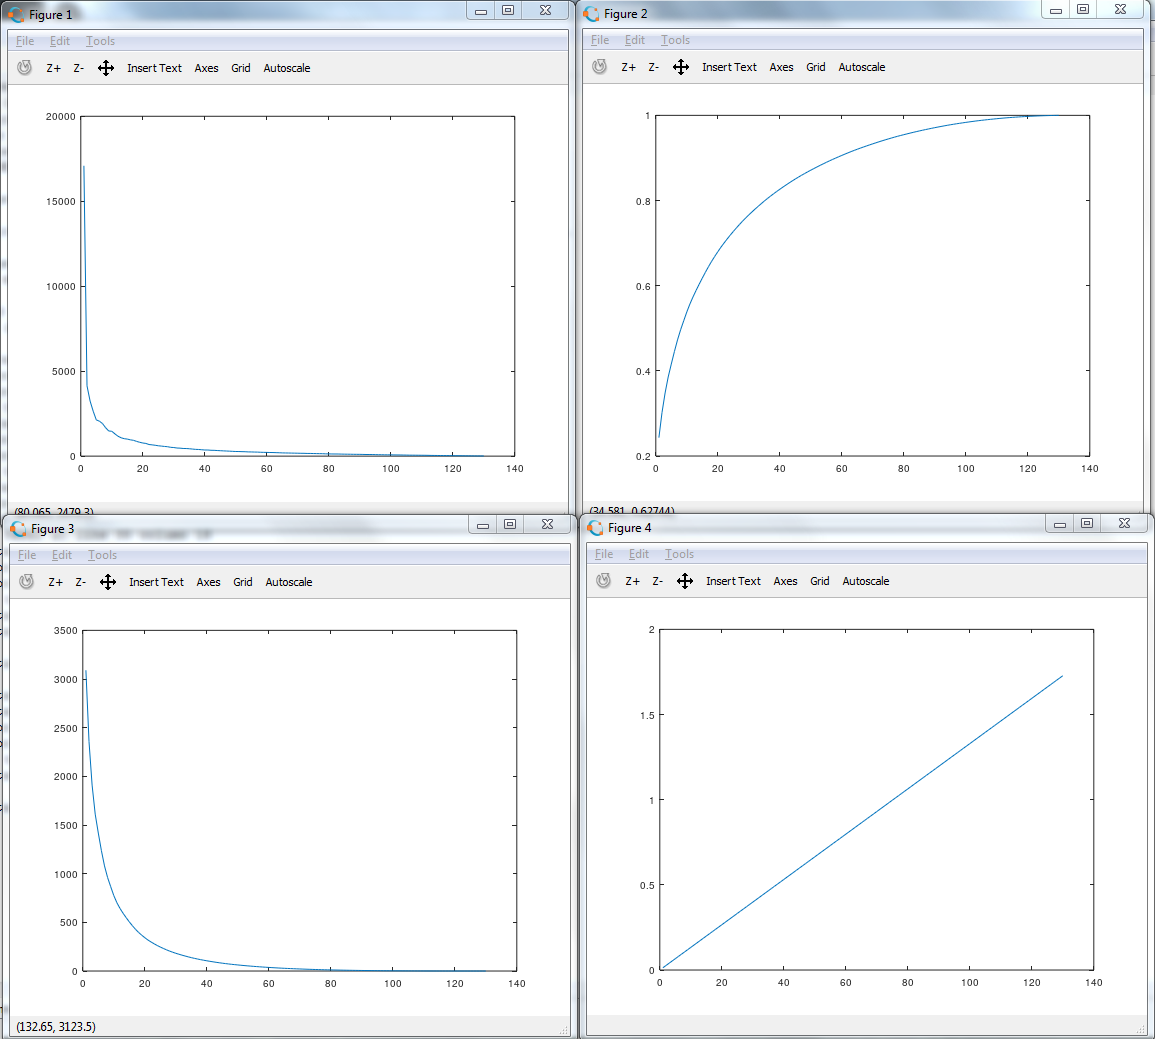
\includegraphics[width=80mm]{grafice_task2_imaginea3.png}
\end{center}
\bigbreak
\title{\textit{graficele rezultate in urma analizei imaginii $4$ din setul de imagini \\}
\begin{center}
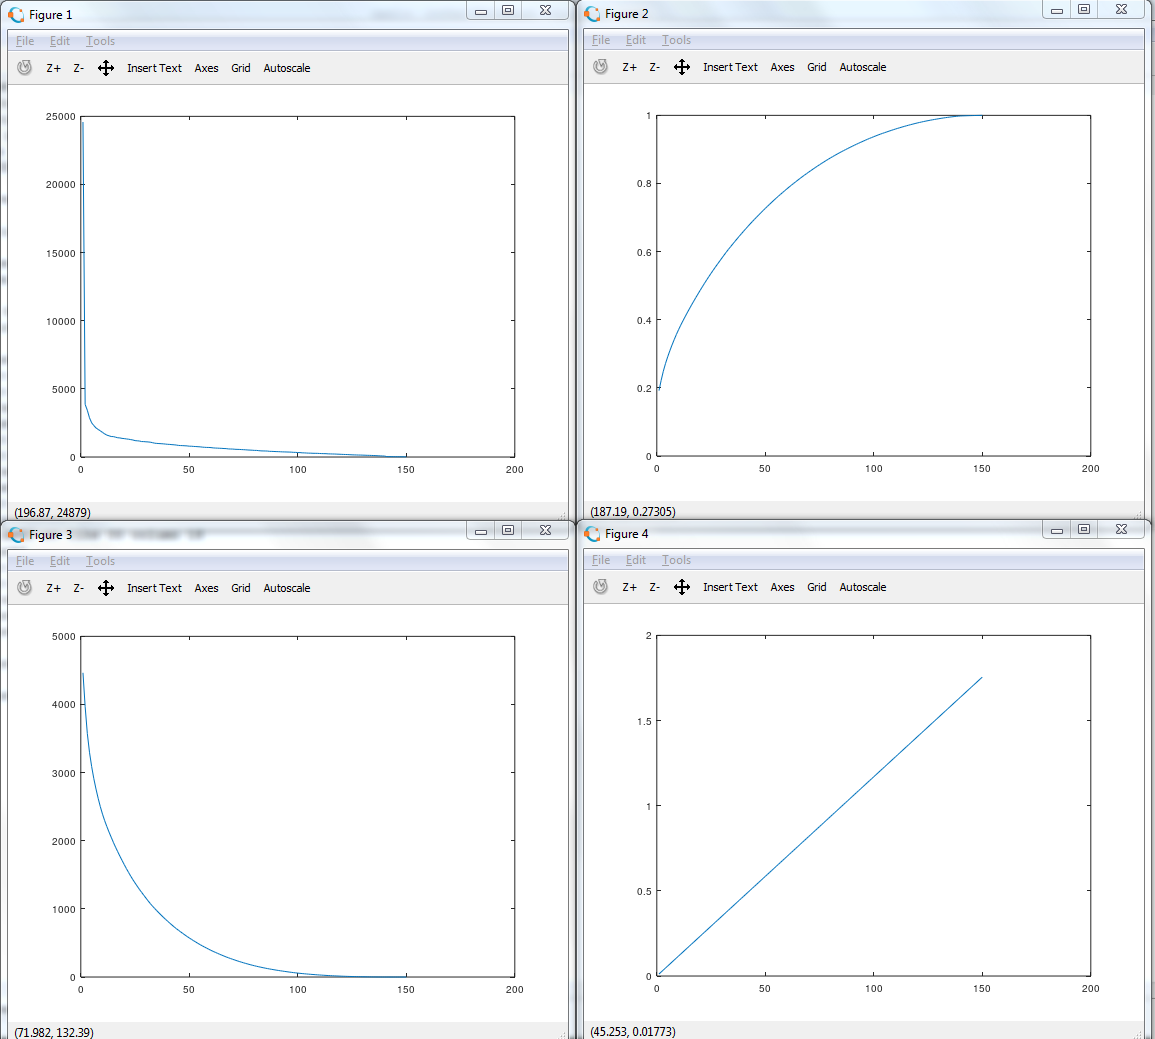
\includegraphics[width=80mm]{grafice_task2_imaginea4.png}
\end{center}

\section{Cerinta 3}
\paragraph{}
Am urmat pasii prezentati in cerinta pentru obtinerea imaginii cerute: am citit
imaginea ceruta, am calculat media pe fiecare linie, am reactualizat matricea
initiala, am construit matricea Z (matricea de covarianta), am calculat DVS pentru matricea Z, am obtinut
spatiul k-dimensional al componentelor principale, am proiectat matricea A in
spatiul componentelor principale si am aproximat matrice initiala.

\section{Cerinta 4}
\paragraph{}
Pasii de inceput si de final sunt asemanatori cu cei de la Cerinta 3, singurele
diferente fiind: calcularea matricii de covarianta, descompunerea eig a aceste-
ia si calcularea spatiului k-dimensional al componentelor principale.

\section{Cerinta 5}
\paragraph{}
Am creat cate o figura diferita pentru fiecare din cele 4 grafice cerute. La
primul, al treilea si ultimul grafic am folosit functia implementata la Cerinta
3, iar la al doilea grafic am folosit descompunerea svd(). Imaginile cu graficele rezultate sunt urmatoarele:
\bigbreak
\title{\textit{graficele rezultate in urma analizei imaginii $3$ din setul de imagini \\}
\begin{center}
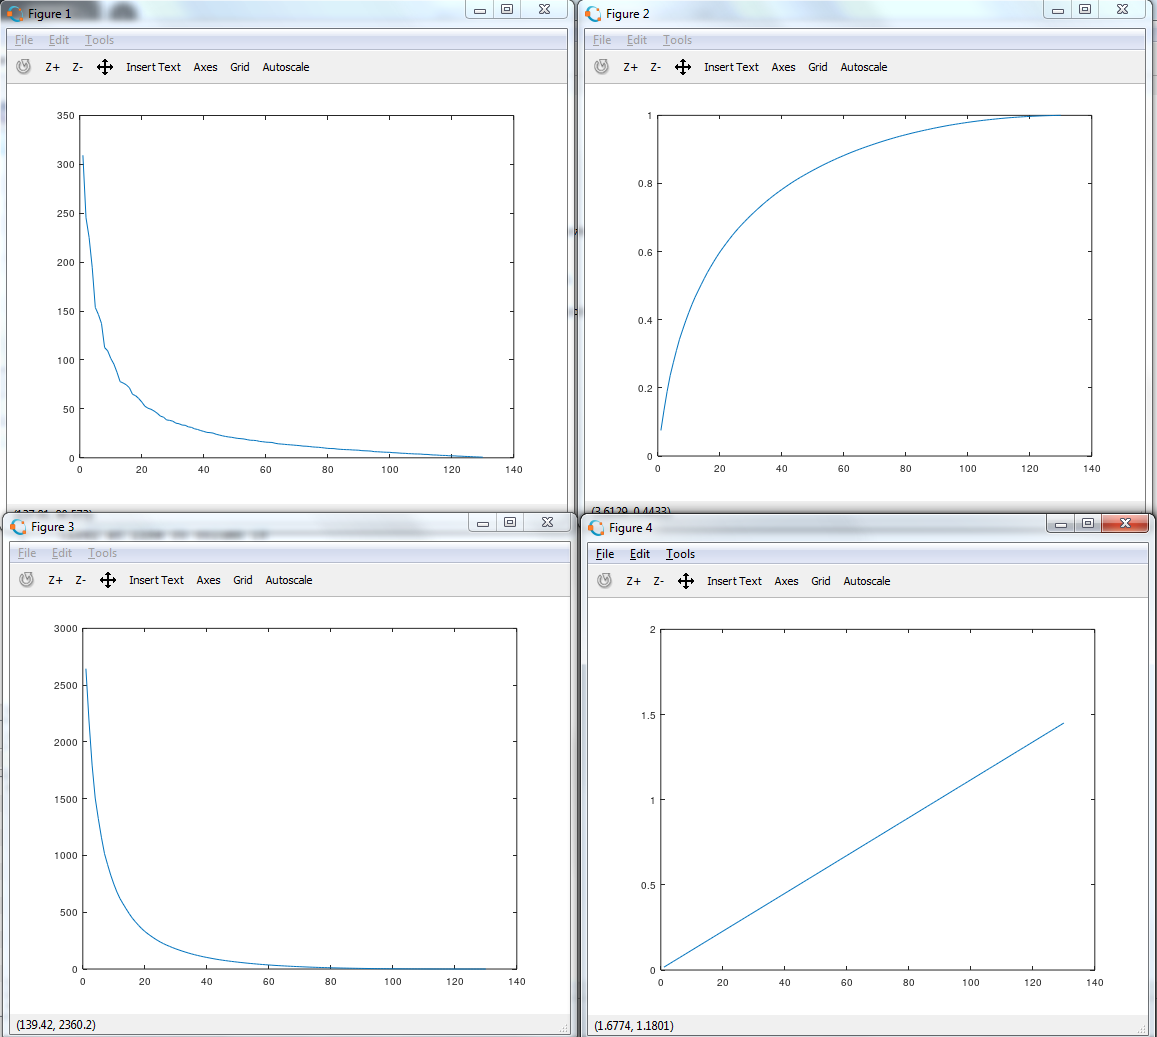
\includegraphics[width=80mm]{grafice_task5_imaginea3.png}
\end{center}
\bigbreak
\title{\textit{graficele rezultate in urma analizei imaginii $4$ din setul de imagini \\}
\begin{center}
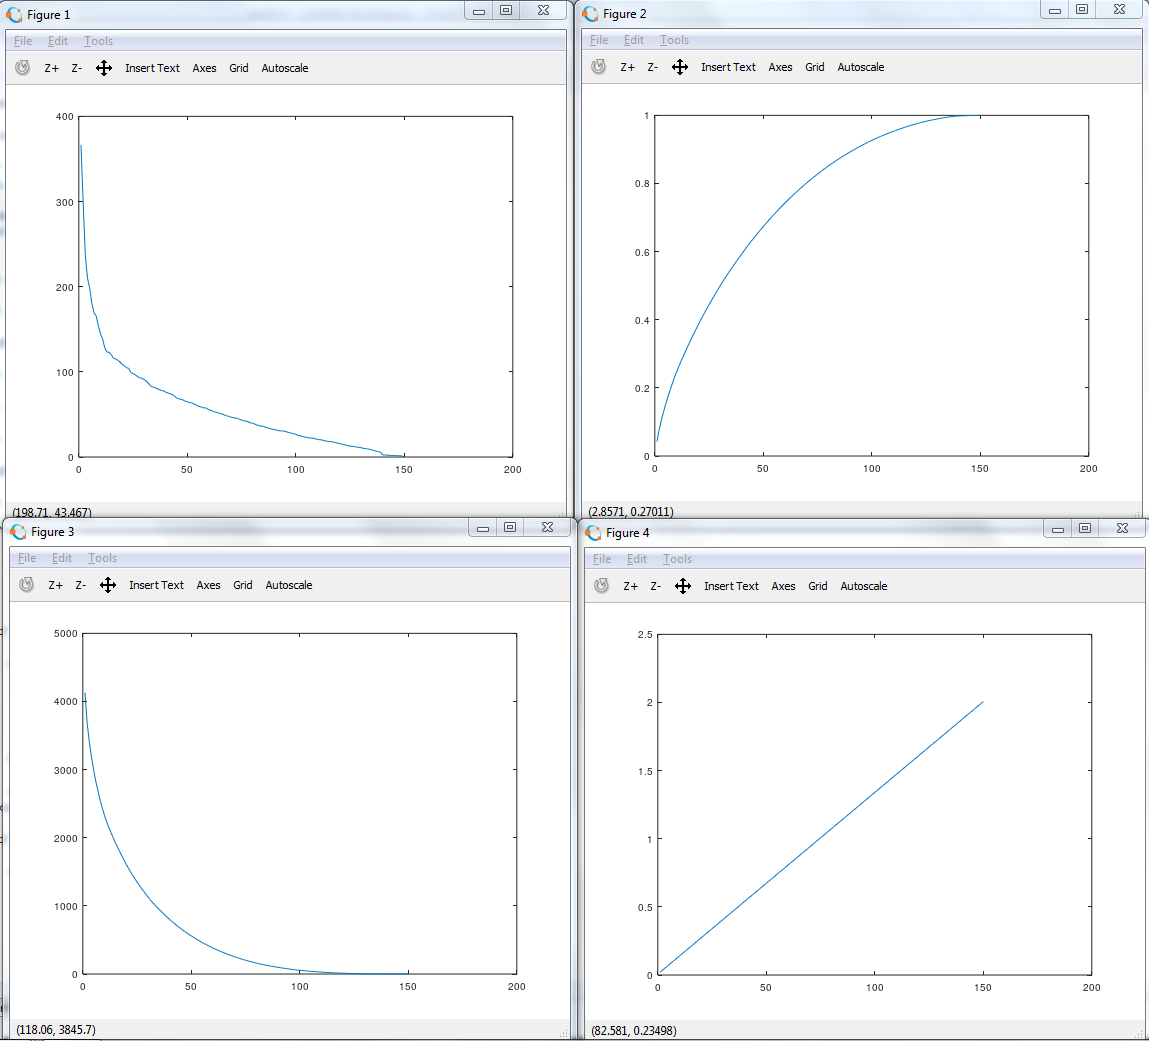
\includegraphics[width=80mm]{grafice_task5_imaginea4.png}
\end{center}

\section{Cerinta 6}
\paragraph{}
Am urmat urmatorii pasi: am citit fiecare imagine intr-o matrice pe care mai
apoi am transformat-o intr-un vector coloana; toate coloanele le-am pus intr-o
matrice care va avea dimensiunea de 40.000 x 10; am calculat media pe fiecare
linie a acestei matrici si mai apoi am 'actualizat' matricea initiala; am des-
compus matricea folosind eig()(am incercat si cu svd() si merge la fel de bine)
; am pus intr-o matrice toti vectorii proprii corespunzatori valorilor proprii
mai mari ca 1 rezultate din descompunere; am calculat matricea cu fetele proprii
si am calculat proiectia fiecarei imagini in spatiul fetelor. Pentru o imagine
de test, am calculat vectorul coloana aferent imaginii, din el scazand media
rezultata anterior; am calculat proiectia imaginii de test in spatiul fetelor si
am cautat cea mai mica distanta dintre proiectia imaginii de test si proiectiile
calculate anterior.

\bigbreak
\title{\underline{Precizari}}
\paragraph{} Pentru anumite grafice de la task-urile 2 si 5, rularea functiei dureaza putin
mai mult pentru ca au loc foarte multe iteratii (in special la graficul care
presupune calcularea erorii aproximative).

\end{document}